\documentclass[11pt]{article}

\usepackage[T1]{fontenc}
\usepackage[polish]{babel}
\usepackage[utf8]{inputenc}
\usepackage{lmodern}
\selectlanguage{polish}

\usepackage{graphicx}
\usepackage{float}
\usepackage{listings}

\graphicspath{{img/}}

\lstset{
	showspaces=false,
    showstringspaces=false,
    frame=single
}

\begin{document}

\thispagestyle{empty}

\noindent
Mateusz Burniak 218321 \\
Krzysztof Cyran 218405 \\
grupa: śr/11/TN

\vfill

\begin{center}
  \begin{Huge}
    Urządzenia Cyfrowe \\
    i Systemy Wbudowane: \\
    \vspace{.5cm}
    projekt
  \end{Huge}
  
  \vspace{3cm}
  
  \begin{Large}
    Gra w labirynt na VGA \\
    z użyciem drążka sterowego
  \end{Large}
  
  \vspace{3cm}
  
  \begin{Large}
    Prowadzący: \\
    dr inż. Jarosław Sugier
  \end{Large}
  
  \vspace{3cm}
  
  Data oddania projektu: \\
  31 V 17
  
\end{center}

\vfill

\newpage

\section{WSTĘP}

\section{OPIS}

\begin{figure}[H]
\center
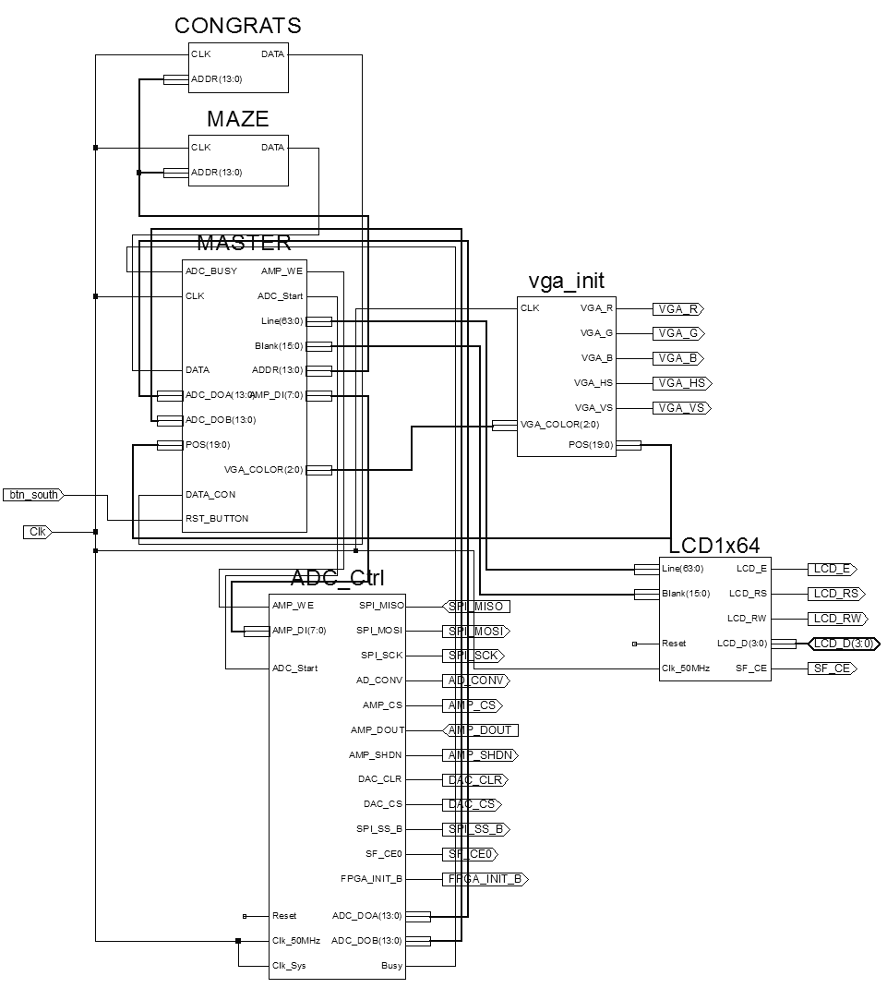
\includegraphics[scale=.6]{schemat.png}
\caption{Schemat całego projektu}
\end{figure}

Powyższy rysunek to schemat projektu.
Widać na nim wszystkie stworzone moduły.

Nasz projekt ma strukturę gwiazdzistą, gdyż każdy moduł połączony jest z modułem głównym MASTER.

\subsection{MASTER}

\begin{figure}[H]
\center
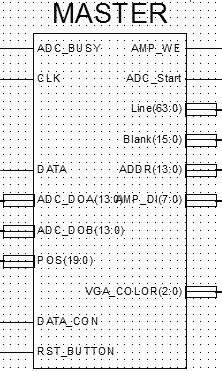
\includegraphics[scale=1]{MASTER.png}
\caption{Schemat modułu MASTER}
\end{figure}

Moduł MASTER odpowiada za całą logikę gry.
Komunikuje się ze wszystkimi innymi modułami.

Znajdują się w nim sygnały wewnętrzne, które zawierają aktualną pozycję kwadratu i aktualnego piksela, jak również inne, potrzebne do liczenia upływającego czasu.

20-bitowy wektor wejściowy POS dzielony jest po 10 bitów na pozycję w pionie i poziomie do sygnałów wewnętrznych HPOS i VPOS.

\begin{lstlisting}
HPOS <= signed('0' & POS(19 downto 10));
VPOS <= signed('0' & POS(9 downto 0));
\end{lstlisting}

Moduł MASTER steruje również wzmocnieniem odbiornika analogowego, wysyłając impulsy na AMP\_WE i ADC\_Start w odpowiednich momentach.
%TODO ref

\begin{lstlisting}
AMP_WE <= '1' when HPOS = 0 and VPOS = 0 else '0';
AMP_DI <= X"22";
ADC_Start <= '1' when HPOS = HMAX and
             VPOS = VMAX else '0';
\end{lstlisting}

MASTER przesyła dane na wyświetlacz LCD, czyli ustawia które pola wyświetlacza mają być zapalone i jakie znaki mają się wyświetlać.
Są to odczyty z wejścia analogowego i aktualny czas gry.

\begin{lstlisting}
Blank <= X"0C30";
Line <= ADC_DOA & "00" & X"00" &
        ADC_DOB & "00" & X"00" &
        STD_LOGIC_VECTOR(PLAYTIME);
\end{lstlisting}	

Kolejnym zadaniem, które wykonuje moduł MASTER to przygotowanie adresu do zapytania pamięci ROM z modułu MAZE.
Ma to na celu sprawdzenie, czy aktualny piksel należy do labiryntu, czy jest tłem.
Po zakończeniu gry wartości pobierane są z pamięci ROM modułu CONGRATS.

\begin{lstlisting}
ADDR <= STD_LOGIC_VECTOR(VPOS(9 downto 3)) &
        STD_LOGIC_VECTOR(HPOS(9 downto 3));
\end{lstlisting}

Jeśli aktualny piksel jest wewnątrz kwadratu, to MASTER ustawia jego kolor na kolor fuksji.
Jeśli jest ścianą labiryntu, to ustawia jego kolor na niebieski.
W innym przypadku ustawianym kolorem jest kolor żółty.
Po skończonej grze kolory pikseli brane są z moduły CONGRATS.

\begin{lstlisting}
VGA_COLOR_INT <= DATA_CON & DATA_CON & not DATA_CON
                 when TIMER_EN = '0'
                 else B"101" when HPOS > BOX_HPOS and
                     HPOS < BOX_HPOS + SIDE and
                     VPOS > BOX_VPOS and
                     VPOS < BOX_VPOS + SIDE
                 else DATA & DATA & not DATA;

\end{lstlisting}

W procesie TIMER obliczany jest czas gry z dokładnością do 0.1 sekundy. 
Jeśli ustawiona jest flaga TOUCHING, to naliczana jest kara czasowa.

\begin{lstlisting}
if TOUCHING = '1' and TIMER_EN = '1' then
    PLAYTIME <= PLAYTIME + 1;
end if;
\end{lstlisting}

Ważnym elementem modułu MASTER jest obsługa przycisku RESET, zerującego pomiar czasu gry oraz pozycję poruszanego kwadratu. 
Przycisk ten działa zarówno w trakcie, jak i po ukończeniu rozgrywki. 

\begin{lstlisting}
process (CLK)
begin
   if rising_edge(CLK) then
      if RST_BUTTON = '1' then
         RESTART <= '1';
      else
         RESTART <= '0';
      end if;
   end if;
end process;
\end{lstlisting}

Najważniejszym elementem modułu MASTER jest proces BOX. 
Odpowiada on za aktualizacje pozycji sterowanego przez drążek sterowy kwadratu w kolorze fuksji.
Do aktualnej pozycji kwadratu dodawane są trzy najstarsze bity otrzymane z kontrolera analogowo-cyfrowego.
Zapewnia to płynność ruchu.

\begin{lstlisting}
if HPOS = 0 and VPOS = 0 then
  BOX_HPOS <= BOX_HPOS - signed(ADC_DOA(13 downto 11));
  BOX_VPOS <= BOX_VPOS + signed(ADC_DOB(13 downto 11));
end if;
\end{lstlisting}


Kwadrat nie ma możliwości wyjśc poza planszę lub wejśc w ścianę labirytnu.

\begin{lstlisting}
if BOX_HPOS < 0 then
    BOX_HPOS <= to_signed(0, 11);
elsif BOX_HPOS > HMAX - SIDE then
    BOX_HPOS <= HMAX - SIDE;
end if;

if BOX_VPOS < 0 then
    BOX_VPOS <= to_signed(0, 11);
elsif BOX_VPOS > VMAX - SIDE then
    BOX_VPOS <= VMAX - SIDE;
end if;
\end{lstlisting}

Próba wejścia w ścianę powoduje ustawienie flagi TOUCHING i odjęcie wartości, która została wcześniej dodana.

\begin{lstlisting}
if TOUCHING = '1' then
  TOUCHING <= '0';
  BOX_HPOS <= BOX_HPOS + signed(ADC_DOA(13 downto 11));
  BOX_VPOS <= BOX_VPOS - signed(ADC_DOB(13 downto 11));
end if;

TOUCHING <= '0';
if DATA = '0' and
  HPOS > BOX_HPOS and HPOS < BOX_HPOS + SIDE and 
  VPOS > BOX_VPOS and VPOS < BOX_VPOS + SIDE then
  TOUCHING <= '1';
end if;
\end{lstlisting}

Kiedy pozycja kwadratu spełnia warunki końcowe, to dezaktywowana jest flaga TIMER\_EN, która zatrzymuje pomiar czasu.

\begin{lstlisting}
if BOX_VPOS < 2 then
   TIMER_EN <= '0';
end if;
\end{lstlisting}



\subsection{vga\_init}

\begin{figure}[H]
\center
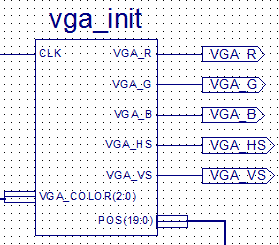
\includegraphics[scale=1]{VGA_init.png}
\caption{Schemat modułu vga\_init}
\end{figure}

Moduł vga\_init oblicza timingi, które wymagane są przez standard VGA.
Jego wyjściem jest pozycja aktualnego piksela zapisana jako 20 bitowy wektor.
Moduł ten jako wejście przyjmuje 3 bitowy numer koloru, który ma wyświetlić na pikselu.
Dodatkowo połączony jest z zewnętrznymi pinami Spartana.

Wewnątrz znajdują się dwa liczniki modulo liczące w górę.
Pierwszy z nich odlicza pozycję w poziomie w sygnale HPOS i kiedy osiąga wartość maksymalną, aktywuje impuls VGA\_HS.
\begin{lstlisting}
HPOS_CNT: process (CLK) 
begin
   if rising_edge(CLK) then
     if HPOS = HPOS_MAX then
         HPOS <= 0;
      else
         HPOS <= HPOS + 1;
      end if;
   end if;
end process HPOS_CNT;
\end{lstlisting}
Drugi licznik zwiększa pozycję w pionie w sygnale VPOS, kiedy licznik HPOS osiąga wartość maksymalną i odpowiada za przeniesienie aktualnego piksela na początek ekranu aktywując VGA\_VS.
\begin{lstlisting}
VPOS_CNT: process (CLK) 
begin
   if rising_edge(CLK) and HPOS = HPOS_MAX then
      if VPOS = VPOS_MAX then
         VPOS <= 0;
      else
         VPOS <= VPOS + 1;
      end if;
   end if;
end process VPOS_CNT;
\end{lstlisting}

Sygnał wyjściowy POS jest konkatenacją 10-bitowych wektorów HPOS i VPOS. 
Kierowany jest do modułu MASTER.
\begin{lstlisting}
POS <= STD_LOGIC_VECTOR(to_unsigned(HPOS, 10)) &
       STD_LOGIC_VECTOR(to_unsigned(VPOS, 10));
\end{lstlisting}


Kolory ustawiane są poprzez sygnały wyjściowe VGA\_R, VGA\_G, VGA\_B.
\begin{lstlisting}
VGA_R <= VGA_COLOR(2) when
         HPOS < HT_DISP and VPOS < VT_DISP else '0';
VGA_G <= VGA_COLOR(1) when
         HPOS < HT_DISP and VPOS < VT_DISP else '0';
VGA_B <= VGA_COLOR(0) when
         HPOS < HT_DISP and VPOS < VT_DISP else '0';
\end{lstlisting}
Pobierane są z 3-bitowego wektora VGA\_COLOR jeśli aktualna pozycja piksela mieści się w widzialnym zakresie monitora.
W przeciwnym wypadku ustawiany jest kolor czarny "000".
\begin{lstlisting}
VGA_HS <= '1' when HPOS >= HT_DISP + HT_FP and
          HPOS < HPOS_MAX - HT_BP else '0';
VGA_VS <= '1' when VPOS >= VT_DISP + VT_FP and
          VPOS < VPOS_MAX - VT_BP else '0';
\end{lstlisting}

\subsubsection{SYMULACJA}

Przeprowadzona została symulacja zachowania modułu vga\_init, na której widać, jak zmienia się wektor pos pod wpływem upływania czasu.

\begin{figure}[H]
\center
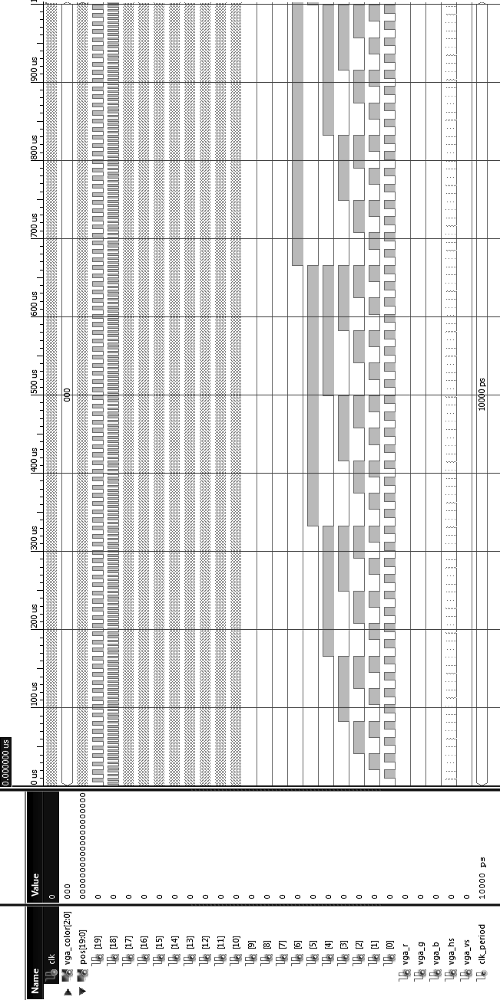
\includegraphics[scale=.5]{symulacja_vga.png} 
\caption{Symulacja modułu vga\_init}
\end{figure}

\subsection{ROM}

\begin{figure}[H]
\center
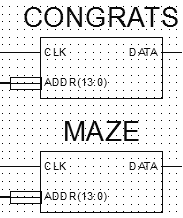
\includegraphics[scale=1]{ROM.png} 
\caption{Schemat pamięci ROM}
\end{figure}

Pamięci ROM są kluczowymi elementami projektu. Występują dwie instancje pamięci tego typu, które są bitmapami o rozmiarze 100x75 zapisanymi jako monochromatyczne bity.
Pierwsza z nich, MAZE, to zapis struktury labiryntu.
Druga to plansza końcowowa z napisem "CONGRATULATION".

\begin{lstlisting}
entity MAZE is
port (CLK : in std_logic;
      ADDR : in std_logic_vector(13 downto 0);
      DATA : out std_logic);
end MAZE;

architecture syn of MAZE is
    type rom_type is array (0 to 9599) of std_logic;
    constant ROM : rom_type:= (
        '0','0','1','1','1','1','1','1', ...
    );

    signal rdata : std_logic;
begin
    rdata <= ROM(conv_integer(ADDR));

    process (CLK)
    begin
        if (rising_edge(CLK)) then
            DATA <= rdata;
        end if;
    end process;
end syn;
\end{lstlisting}

Na powyższym fragmencie kodu pamięci ROM zapisane jest 9600 bitów, które odpowiadają blokom pikseli 8x8.
Piksele zostały tak zgrupowane w celu zaoczędzenia pamięci, kosztem widzianej rozdzielczości.
Pamięć ROM na wejściu przyjmuje 14-bitowy wektor, który jest adresem komórki pamięci.
Starsze 7 bitów to numer wiersza, a młodsze to numer kolumny.
//
Pomimo, że na ekranie o rozdzielczości 800x600 można wyświetlić 7500 bloków 8x8-bitowych, to dodane zostało 28 kolumn, które są niewidoczne na ekranie, ale ułatwiają adresację w pamięci.
Dzieje się tak, ponieważ liczby w zakresie 100+28 można zapisać na dokładnie 7 bitach.
% TODO

\subsection{POZOSTAŁE MODUŁY}

\begin{figure}[H]
\centering
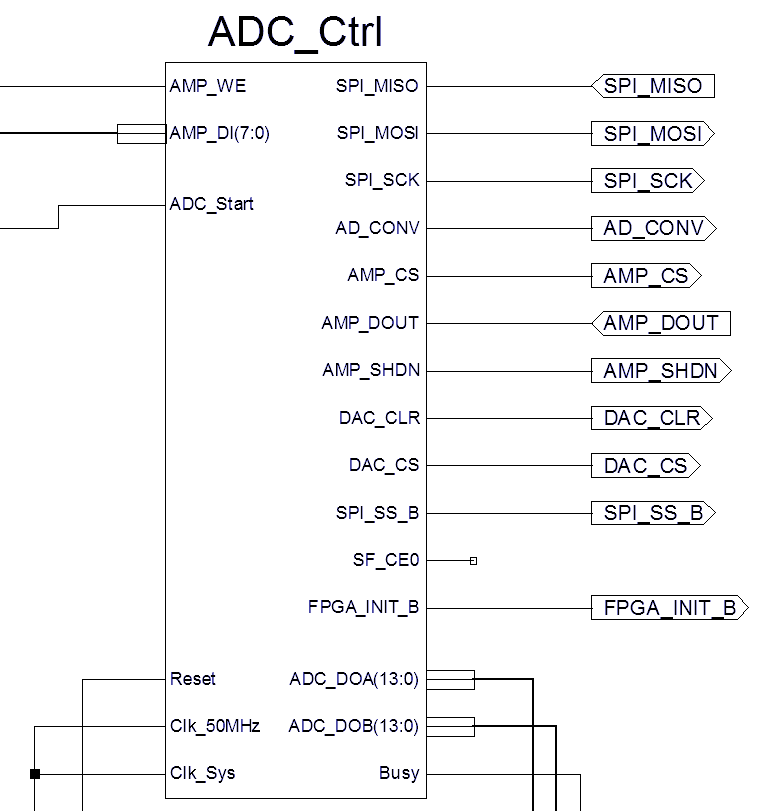
\includegraphics[scale=.5]{ADC_Ctrl.PNG}
\caption{Schemat modułu ADC\_Ctrl}
\end{figure}

\begin{figure}[H]
\centering
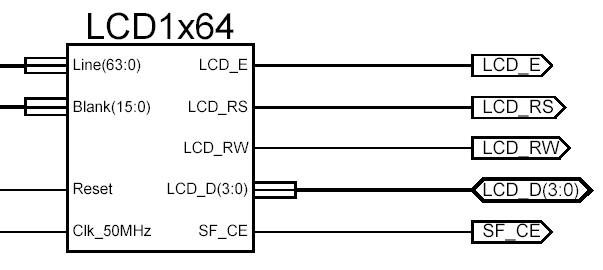
\includegraphics[scale=.5]{LCD1x64.PNG}
\caption{Schemat modułu LCD1x64}
\end{figure}

W projekcie użyte zostały również inne moduły, których kod jest nieznany.
Są to ADC\_Ctrl i LCD1x64.
Pierwszy odpowiada za sczytywanie syganłów analogowych z drążka sterowego i przekazanie do modułu MASTER jego pozycji w postaci cyfrowej.
Drugi moduł komunikuje się z wyświetlaczem LCD i wyświetla na nim pozycje drążka w pionie i poziomie oraz aktualny czas gry.
Traktowane są jako czarne skrzynki, dla których zdefiniowane są wejścia i wyjścia.
Więcej na ten temat można znaleźć na stronie 
% TODO


\section{IMPLEMENTACJA}

\subsection{WYKORZYSTANIE SPRZĘTU}

Poniższa tabela przedstawia wybrane parametry użycia Spartana-3E.
Wynika z niej, że projekt używa niewielki procent dostępnych zasobów.


\begin{tabular}{|l|l|l|l|}
\hline
Logic Utilization &
Used &
Available &
Utilization \\
\hline
Number of Slice Flip Flops &
236 &
9,312 &
2\% \\
\hline
Number of 4 input LUTs &
369 &
9,312 &
3\% \\
\hline
Number of occupied Slices &
286 &
4,656 & 
6\% \\
\hline
Number of Slices containing only related logic &
286 &
286 &
100\% \\
\hline

Total Number of 4 input LUTs &
470 &
9,312 &
5\% \\
\hline
Number used as logic &
368 & & \\
\hline
 
Number used as a route-thru &
101 & & \\
\hline
 
Number used as Shift registers &
1 & & \\
\hline
 
Number of bonded IOBs &
27 &
232 &
11\% \\
\hline
Number of IDDR2s used &
1 & & \\
\hline 
 
Number of ODDR2s used &
2 & & \\
\hline
 
 
Number of RAMB16s &
2 &
20 &
10\% \\
\hline
Number of BUFGMUXs &
1 &
24 &
4\% \\
\hline
Average Fanout of Non-Clock Nets &
2.98 & & \\
\hline
\end{tabular}

\vspace{1em}

Ograniczenia czasowe wyglądają następująco.
Użyty został zegar o okresie 20 ns.
Narzędzie Xilinx ISE wygenerowało raport, z którego wynika, że Worst Case Slack dla SETUP wynosi 2,590 ns, a dla HOLD 0,968 ns.
Wartości dodatnie oznaczają, że ograniczenia są spełnione.
Best Case Achievable jest dostępny tylko dla czasu SETUP i jest równy 14,820 ns.

Podczas generowania raportu nie zostały znalezione żadne błędy związane z zegarem.


\subsection{PODRĘCZNIK UŻYTKOWNIKA}

Poniższy podręcznik użytkownika ma na celu krótkie wprowadzenie do obsługi gry, bez zagłębiania się w szczegóły implementacyjne.

Celem gry jest przejście labiryntu kwadratem przy pomocy drązka sterowego w jak najkrótszym czasie. Za dotknięcie ściany naliczana jest kara czasowa w postaci wielokrotnie przyspieszonego liczenia czasu.

\begin{figure}[H]
\centering
\includegraphics[scale=.5]{plytka.jpg}
\caption{Płytka z potrzebnym sprzętem}
\end{figure}

A - wyjście podłączenia monitora przez port VGA \\
B - wejście analogowe do podłączenie drążka sterowego \\
C - analogowy drążek sterowy \\
D - wyświetlacz LCD \\
E - przycisk resetu \\

Jak widać na zdjęciu wtyczka od drążka sterowego musi być podłączona do pinów po prawej stronie i zwrócona widocznymi blaszkami na zewnątrz.

Przed rozpoczęciem gry należy drążek ustawić możliwie w pozycji pionowej.
Oprócz tego należy zwrócić uwagę na to, by osie drążka odpowiadały układowi współrzędnych, gdzie wartości osi X rosną w prawo, a osi Y w górę.
Ma to na celu poprawne odzwierciedlenie ruchów gracza w grze. 
%

Po podłączeniu potrzebnego osprzętu i zaprogramowaniu płytki gra rozpoczyna się. 

\begin{figure}[H]
\centering
\includegraphics[scale=.5]{game.jpg}
\caption{Widok labiryntu podczas gry}
\end{figure}

Kwadrat w kolorze fuksji, którym poruszamy za pomocą drążka sterowego znajduje się lewym, dolnym rogu.
Gracz poprzez manewrowanie drążkiem sterowym kontroluje ruch kwadratu.
Poruszać się można tylko po żółtym polu. Ściany labiryntu reprezentowane są kolorem niebieskim.

\begin{figure}[H]
\centering
\includegraphics[scale=.5]{end-screen.jpg}
\caption{Widok końcowy gry}
\end{figure}

Koniec labiryntu znajduje się w lewym, górnym rogu.
Po dojściu tam, pokazuje się grafika końcowa z napisem CONGRATULATION. %rys. end-screen
Ponadto zatrzymywany jest pomiar czasu, który pokazany jest na wyświetlaczu LCD po prawej stronie w systemie szesnastkowym.
W celu rozpoczęcia nowej rozgrywki należy użyć przycisku RESET.





\section{PODSUMOWANIE}

Po zakończeniu prac można krytycznie ocenić realizację założeń projektu.
Wszystkie z początkowo postawionych celów zostały spełnione w planowanym terminie, dlatego jesteśmy zadowoleni z ogółu wyników prac.
Pewne rozwiązania, które przyjęliśmy na początku okazały się jednak chybione i po wielogodzinnych analizach problemu oraz pomocy prowadzącego, musieliśmy diametralnie je zmienić.
Przykład może stanowić użycie danych typu integer.
Choć zachęcające prostotą użycia, sprawiły nie lada problem dla sprzętu.
Okazało się, że należy skorzystać z typu signed.

Kolejną trudnością było przejście z architektury jednomodułowej do wielomodułowej.
Zmiana ta spowodowana była nieczytelnością projektu.
Zbyt wiele procesów w jednym module utrudniało analizę przepływu informacji.
Rozwiązaniem tego problemu było wprowadzenie modułu MASTER, który jako moduł główny łączył pozostałe moduły.
W tym przypadku problematyczne było przeniesienie procesów do MASTERa i dostrojenie ich.

Analizując przebieg prac na projektem, dochodzimy do wniosku, że było kilka elementów, które dałoby się poprawić.
Gdybyśmy jeszcze raz realizowali ten projekt, to od razu dzielilibyśmy system na więcej modułów, by uniknąć problemów przy zmianie.
Ponadto logika sterowania kwadratem również mogłaby być osobnym modułem, co odchudziłoby moduł MASTER.

\subsection{KIERUNKI DALSZYCH PRAC}

Po zakończeniu projektu, pomimo pełnej założonej funkcjonalności, możemy określić dalsze kierunki rozwoju gry.
Przede wszystkim można zaimplementować nowe mapy labiryntów, o rosnącym poziomie trudności, by gra była coraz większym wyzwaniem.
Kolejny pomysł to możliwość zmiany kolorów w grze za pomocą przycisków, które znajdują się dookoła potencjometru na płytce Spartan 3E.
Można również rozbudować projekt o kolejne urządzenia peryferyjne, takie, jak głośnik, na którym odtwarzana byłaby muzyczka umilająca grę.
Następny pomysł, to dodanie obsługi kolejnego drążka sterowego, w celu możliwości gry wieloosobowej na jednym monitorze.
W ten sposób element rywalizacji osiągnąłby wyższy poziom.
Ostatnia propozycja to zapisywanie rankingu czasów osiągniętych przez graczy.


\section{SPIS LITERATURY}

ąćęłóńźżś

\end{document}
